\documentclass[border={10pt}]{standalone}
\usepackage{tikz}
\usetikzlibrary{patterns}

\begin{document}

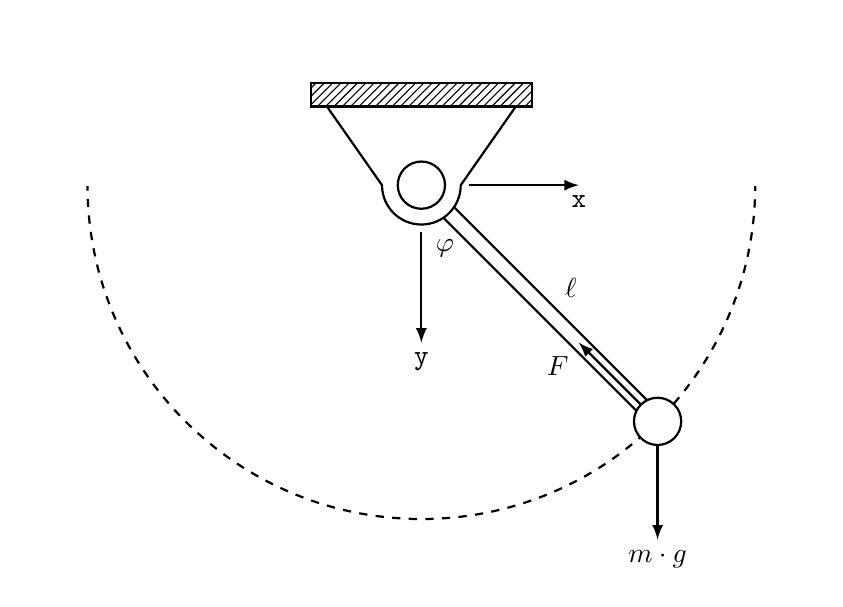
\begin{tikzpicture}[thick,>=latex,->]

\begin{scope}
\clip(-5,2) rectangle (5,-5);

\draw[dashed] (0,0)  circle (4.24cm);
\filldraw[white] (-4.3,4.3) rectangle (4.3,0);
\draw[double distance=1.6mm] (0,0) -- (3,-3) node[midway,xshift=4mm,yshift=2mm]{$\ell$};
\draw[->] (3,-3) -- (3,-4.5) node[below]{$m\cdot g$};
\draw[->] (3,-3) -- (2.,-2.0) node[left,yshift=-3mm]{$F$};
\draw[fill=white] (-1.2,1.0) -- (-.5,0) arc(180:360:0.5) -- (1.2,1.0) -- cycle;
\draw[draw=black,fill=white] (0, 0) circle circle (.3cm);
\draw[draw=black,fill=white] (3,-3) circle circle (.3cm);
\draw[->] (.6,0) -- (2,0) node[below]{\texttt{x}};
\draw[->] (0,-.6) -- (0,-2) node[below]{\texttt{y}};
\draw[pattern=north east lines] (-1.4,1.3) rectangle (1.4,1);
\node at (.3,-.8) {$\varphi$};   
\end{scope}

\end{tikzpicture}
\end{document}